\documentclass[multi=tikzpicture,border=7pt]{standalone}
\usepackage{ctex,amsmath,bm}
\usepackage{tikz}
\usetikzlibrary{arrows.meta,calc,angles,quotes,decorations.pathmorphing,patterns,positioning,intersections}
\tikzset{
axis/.style={->,>=Stealth,thick},force/.style={->,>=Stealth,very thick},
flow/.style={->,>=Stealth,thick,blue!70!black},dim/.style={<->,>=Stealth,thin},
body/.style={draw=black,fill=blue!7,thick},guide/.style={text=black,dashed,gray!70,text=black},
point/.style={circle,fill=black,inner sep=1.5pt},field/.style={->,>=Stealth,thick,purple!75!black},
panel/.style={font=\bfseries,anchor=west},
callout/.style={draw=gray!65,rounded corners,fill=white,align=center,inner sep=3pt}}
\begin{document}

% 01 question-01
\begin{tikzpicture}[x=.88cm,y=.88cm]
  \begin{scope}[shift={(-4.7,0)}]
    \node[panel] at (-3.0,4.05){(a) 竖直洞口的反复踩压};
    \draw[very thick] (-2.8,0)--(-.9,0) (.9,0)--(2.8,0);
    \foreach \x in {-2.6,-2.3,...,-1.0,1.0,1.3,...,2.6}{\draw[thin] (\x,0)--++(-.16,-.18);}
    \draw[very thick] (-.9,.05)--(-.9,-2.65)--(.9,-2.65)--(.9,.05);
    \draw[body,fill=brown!18] (-.9,-.16) rectangle (.9,.16);
    \node[anchor=west] at (1.45,.58){轻质木板};
    \node[anchor=west] at (1.08,-2.65){洞底};
    \draw[thick,decorate,decoration={coil,segment length=4.2pt,amplitude=3.2pt}] (0,2.75)--(0,.82);
    \draw[body,fill=orange!25] (-.55,2.75) rectangle (.55,3.15);
    \node[anchor=west,align=left] at (.75,2.95){跳跳虎，质量 $m$\\尾部等效为弹簧 $k$};
    \draw[dim] (-1.55,.18)--(-1.55,2.75) node[midway,left]{$H$};
    \node[anchor=east] at (-1.65,2.75){由静止释放};
    \draw[force,red!75!black] (0,.72)--(0,.2) node[midway,right]{踩压力};
    \draw[guide] (-.9,-.65)--(.9,-.65);
    \draw[dim] (-1.25,-.16)--(-1.25,-.65) node[midway,left]{$d_n$};
    \node[anchor=west,font=\small] at (1.08,-.72){第 $n$ 次踩压后的木板位置};
  \end{scope}
  \begin{scope}[shift={(4.7,-.05)}]
    \node[panel] at (-3.2,4.05){(b) 顶角为 $60^\circ$ 的粗糙 V 形槽};
    \draw[very thick] (-3.0,2.65)--(0,-2.65)--(3.0,2.65);
    \node[rotate=60] at (-2.68,1.55){粗糙槽壁};
    \node[rotate=-60] at (2.68,1.55){粗糙槽壁};
    \draw[very thick,brown!75!black] (-2.12,.83)--(2.12,.83);
    \fill (-2.12,.83) circle(1.8pt); \fill (2.12,.83) circle(1.8pt);
    \node[anchor=north east] at (-2.18,.70){接触点 $L$};
    \node[anchor=north west] at (2.18,.70){接触点 $R$};
    \fill (0,.83) circle(1.6pt) node[below]{$O$};
    \filldraw[fill=orange!35,thick] (.88,.83) circle(.13) node[above left]{$P$};
    \draw[force,red!75!black] (.88,2.05)--(.88,1.02);
    \node[red!75!black,anchor=south] at (.88,2.12){作用力};
    \coordinate (A) at (-3,2.65); \coordinate (V) at (0,-2.65); \coordinate (B) at (3,2.65);
    \draw pic[draw,"$60^\circ$",angle radius=.78cm,angle eccentricity=1.35]{angle=B--V--A};
    \draw[dim] (-2.12,1.48)--(2.12,1.48) node[midway,above]{杆长 $l$};
    \draw[dim] (0,.28)--(.88,.28) node[midway,below]{$x=OP$};
    \node[callout,font=\small] at (0,-3.55){轻杆水平卡在两槽壁之间；$P$ 为随机踩压点};
  \end{scope}
\end{tikzpicture}

% 02 solution-01
\begin{tikzpicture}[x=.84cm,y=.84cm]
  \begin{scope}[shift={(-4.6,0)}]
    \draw[axis] (-.4,0)--(5.2,0) node[right]{$n$};
    \draw[axis] (0,-.3)--(0,4.3) node[above]{$d_n$};
    \foreach \x/\y/\lab in {1/.55/$d_1$,2/1.15/$\frac32d_1$,3/2.15/$\left(\frac32\right)^2d_1$,4/3.55/$\left(\frac32\right)^3d_1$}{
      \draw[blue!65!black,very thick] (\x,0)--(\x,\y); \node[above] at (\x,\y){\lab};}
    \node[draw,rounded corners,fill=blue!8,align=left] at (2.55,-1.35)
      {$d_{n+1}=\dfrac32d_n$\\$D=\sum_{n=1}^{N}d_n$};
  \end{scope}
  \begin{scope}[shift={(4.4,.2)}]
    \draw[very thick] (-2.5,3.925)--(0,-.405)--(2.5,3.925);
    \draw[very thick,brown!70!black] (-1.1,1.5)--(1.1,1.5);
    \fill (-1.1,1.5) circle(2pt); \fill (1.1,1.5) circle(2pt);
    \draw[force,red!75!black] (-1.1,1.5)--++(25:.9);
    \draw[force,red!75!black] (1.1,1.5)--++(155:.9);
    \node[red!75!black,fill=white,inner sep=1.5pt] at (-.55,2.28){$\bm R_L$};
    \node[red!75!black,fill=white,inner sep=1.5pt] at (.55,2.28){$\bm R_R$};
    \draw[force] (.45,1.5)--(.45,.55) node[below right]{$P$};
    \draw[guide] (-1.1,1.5)--++(15:2.3) (-1.1,1.5)--++(45:2.3);
    \draw[guide] (1.1,1.5)--++(135:2.3) (1.1,1.5)--++(165:2.3);
    \node[align=center] at (0,-2.75){接触合力必须落在摩擦锥内\\$\varphi=\arctan\mu$};
  \end{scope}
\end{tikzpicture}

% 03 question-02
\begin{tikzpicture}[x=1cm,y=1cm]
  \node[panel] at (-5.25,4.05){轴承支承的空间转轴与转动连杆};
  \coordinate (O) at (0,0);
  \coordinate (A) at (2.15,1.80);
  \coordinate (B) at (-2.15,-1.80);
  \coordinate (Sleft) at (-3.34,1.35);
  \coordinate (Sright) at (3.34,-1.35);

  % 这是与固定转轴垂直的转动平面；椭圆用于表达透视，而不是圆盘实体。
  \begin{scope}[rotate=68]
    \fill[blue!6,opacity=.70] (0,0) ellipse[x radius=3.35,y radius=.92];
    \draw[guide,dashed] (-3.35,0) arc[start angle=180,end angle=360,x radius=3.35,y radius=.92];
    \draw[gray!72,thick] (3.35,0) arc[start angle=0,end angle=180,x radius=3.35,y radius=.92];
    \draw[red!72!black,very thick,->]
      (-2.65,.55) arc[start angle=168,end angle=58,x radius=3.35,y radius=.92];
  \end{scope}
  \node[red!72!black] at (-2.55,2.15){$\omega$};

  % 固定转轴先画在后层；它穿过 O，并在两侧由轴承支承。
  \draw[black!72,very thick] (-4.45,1.80)--(4.45,-1.80);
  \begin{scope}[shift={(Sleft)},rotate=68]
    \shade[ball color=gray!35] (0,0) ellipse[x radius=.50,y radius=.20];
    \draw[very thick] (0,0) ellipse[x radius=.50,y radius=.20];
  \end{scope}
  \begin{scope}[shift={(Sright)},rotate=68]
    \shade[ball color=gray!35] (0,0) ellipse[x radius=.50,y radius=.20];
    \draw[very thick] (0,0) ellipse[x radius=.50,y radius=.20];
  \end{scope}
  \draw[thick] (-3.34,1.12)--(-3.34,.15)--(-4.02,.15)
               (3.34,-1.58)--(3.34,-2.55)--(4.02,-2.55);
  \draw[thick] (-4.12,.15)--(-3.02,.15) (3.02,-2.55)--(4.12,-2.55);

  % 轮毂与 AB 连杆位于前层；连杆和转轴在 O 处连接但方向不同。
  \shade[ball color=blue!28] (O) circle(.34);
  \draw[black,very thick] (B)--(A);
  \fill (O) circle(2.1pt) node[below right]{$O$};
  \shade[ball color=orange!58] (A) circle(.27);
  \shade[ball color=orange!58] (B) circle(.27);
  \node[above right] at (A) {$A,m$};
  \node[below left] at (B) {$B,m$};
  \draw[dim] (O)--(A) node[midway,above left]{$r$};

  % 小球沿真实竖直方向落下，并在图示瞬间撞击 A。
  \draw[gray!72,thick] (1.96,4.05)--(1.96,3.03);
  \draw[gray!72,thick] (2.34,4.05)--(2.34,3.03);
  \shade[ball color=red!45] (2.15,3.62) circle(.22);
  \node[right] at (2.39,3.62) {$m$};
  \draw[flow] (2.15,3.30)--(2.15,2.15) node[midway,right]{$v$};
\end{tikzpicture}

% 04 solution-02
\begin{tikzpicture}[x=.88cm,y=.88cm]
  \begin{scope}[shift={(-4.5,0)}]
    \draw[axis] (-.4,0)--(5.3,0) node[below left]{$i$};
    \draw[axis] (0,-.3)--(0,4.2) node[above]{$\omega_i r/v$};
    \draw[blue!70!black,very thick]
      plot coordinates {(0,0) (1,2.1333) (2,2.8444) (3,3.0815) (4,3.1605) (5,3.1868)};
    \draw[guide] (0,3.2)--(5,3.2) node[right]{$1$};
    \foreach \x/\y in {0/0,1/2.1333,2/2.8444,3/3.0815,4/3.1605,5/3.1868}
      {\fill (\x,\y) circle(1.5pt);}
    \node at (2.5,-1.0){$\omega_{i+1}=\dfrac13\omega_i+\dfrac23\dfrac vr$};
  \end{scope}
  \begin{scope}[shift={(4.3,.1)}]
    \node[draw,rounded corners,fill=blue!8,align=left] at (0,2.1)
      {轻杆：$\ I=2mr^2$\\等效切向质量：$\ I/r^2=2m$};
    \draw[flow] (0,1.15)--(0,.55);
    \node[draw,rounded corners,fill=orange!10,align=left] at (0,-.1)
      {均质杆 $4m$：\\$I=2mr^2+\frac1{12}(4m)(2r)^2=\frac{10}{3}mr^2$};
    \draw[flow] (0,-1.25)--(0,-1.85);
    \node[draw,rounded corners,fill=green!8,align=left] at (0,-2.4)
      {$\omega_{k+1}=\frac7{13}\omega_k+\frac6{13}\frac vr$};
  \end{scope}
\end{tikzpicture}

% 05 question-03
\begin{tikzpicture}[x={(1cm,0cm)},y={(.55cm,.38cm)},z={(0cm,1cm)}]
  \node[panel] at (-5.0,0,4.25){带电圆环与中轴线上的金属小球};
  \coordinate (O) at (0,0,0);
  \coordinate (P) at ({3.2*cos(32)},{3.2*sin(32)},0);

  % 三维坐标与位于 x-y 平面内的真实圆环。
  \draw[axis] (-4.5,0,0)--(4.7,0,0) node[right]{$x$};
  \draw[axis] (0,-4.0,0)--(0,4.1,0) node[above right]{$y$};
  \draw[axis] (0,0,-2.2)--(0,0,4.45) node[above]{$z$};
  \fill[blue!7,opacity=.58]
    plot[domain=0:360,samples=90,variable=\t] ({3.2*cos(\t)},{3.2*sin(\t)},0) -- cycle;
  \draw[blue!55!black,dashed,thick]
    plot[domain=0:180,samples=50,variable=\t] ({3.2*cos(\t)},{3.2*sin(\t)},0);
  \draw[blue!65!black,very thick]
    plot[domain=180:360,samples=50,variable=\t] ({3.2*cos(\t)},{3.2*sin(\t)},0);
  \foreach \t in {205,235,...,355}{
    \node[blue!65!black,font=\scriptsize] at ({3.2*cos(\t)},{3.2*sin(\t)},0){$+$};}
  \fill (O) circle(2pt) node[below left]{$O$};
  \draw[dim] (O)--(P) node[midway,above]{$R$};
  \node[blue!65!black,anchor=west] at (3.35,-.3,0){线电荷密度 $\lambda$};

  % 小球位于垂直圆环平面的中轴线上，遮挡关系由透视直接表示。
  \draw[guide] (O)--(0,0,2.85);
  \draw[dim] (-.55,0,0)--(-.55,0,2.85) node[midway,left]{$h$};
  \shade[ball color=orange!48] (0,0,2.85) circle(.34);
  \node[anchor=west] at (.55,0,3.05){$Q=0,\ m$};
  \node[anchor=west] at (.55,0,2.62){半径 $r\ll R$};
  \draw[field] (0,0,1.25)--(0,0,2.25) node[midway,right]{$\bm E(h)$};
\end{tikzpicture}

% 06 solution-03
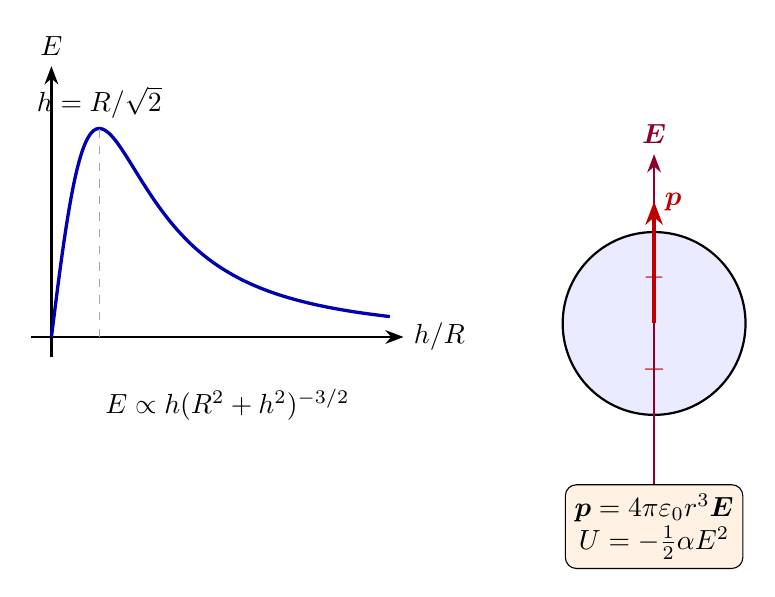
\begin{tikzpicture}[x=.86cm,y=.86cm]
  \begin{scope}[shift={(-4.6,0)}]
    \draw[axis] (-.3,0)--(5.2,0) node[right]{$h/R$};
    \draw[axis] (0,-.3)--(0,4.0) node[above]{$E$};
    \draw[blue!70!black,very thick,domain=0:5,samples=160] plot (\x,{8*\x/(1+\x*\x)^(1.5)});
    \draw[guide] (.707,0)--(.707,3.08) node[above]{$h=R/\sqrt2$};
    \node at (2.6,-1.0){$E\propto h(R^2+h^2)^{-3/2}$};
  \end{scope}
  \begin{scope}[shift={(4.3,.2)}]
    \draw[body,fill=blue!8] (0,0) circle(1.35);
    \node[red!75!black] at (0,.68){$-$}; \node[red!75!black] at (0,-.68){$+$};
    \draw[field] (0,-2.5)--(0,2.5) node[above]{$\bm E$};
    \draw[force,red!75!black] (0,0)--(0,1.8) node[right]{$\bm p$};
    \node[draw,rounded corners,fill=orange!10,align=center] at (0,-3.0)
      {$\bm p=4\pi\varepsilon_0r^3\bm E$\\$U=-\frac12\alpha E^2$};
  \end{scope}
\end{tikzpicture}

% 07 question-04
\begin{tikzpicture}[x=.95cm,y=.95cm]
  \node[panel] at (-5.4,3.0){平行光滑轨道上的碰撞—弹簧耦合系统};
  \draw[very thick] (-5.0,-1.55)--(5.0,-1.55) (-5.0,1.75)--(5.0,1.75);
  \node[anchor=east] at (-5.1,1.75){上轨道}; \node[anchor=east] at (-5.1,-1.55){下轨道};
  \filldraw[fill=orange!28,thick] (-3.35,-1.55) circle(.25) node[below]{$B$，质量 $2m$};
  \filldraw[fill=orange!28,thick] (0,-1.55) circle(.25) node[below]{$A$，质量 $m$};
  \filldraw[fill=orange!28,thick] (0,1.75) circle(.25) node[above]{$D$，质量 $3m$};
  \draw[very thick,decorate,decoration={coil,segment length=4.3pt,amplitude=3.2pt}] (0,-1.28)--(0,1.48);
  \node[callout,anchor=west] at (.55,.1){劲度系数 $k$\\原长可忽略};
  \draw[flow] (-3.02,-.95)--(-.85,-.95) node[midway,above]{$v_0$};
  \draw[red!70!black,very thick,->] (-2.95,-1.55)--(-.42,-1.55) node[midway,below=.45cm]{第一次完全弹性碰撞：$B\to A$};
  \draw[dim] (4.15,-1.55)--(4.15,1.75) node[midway,right]{轨道间距 $d$};
  \node[font=\small,anchor=north] at (0,-3.0){初始时 $A,D$ 静止；三物体只沿各自轨道运动};
\end{tikzpicture}

% 08 solution-04
\begin{tikzpicture}[x=1.8cm,y=1.8cm]
 \draw[axis] (-.1,0)--(3.65,0) node[right]{$\Omega t$};
 \draw[axis] (0,-.15)--(0,1.9) node[above]{$\Omega x/v_0$};
 \draw[blue!70!black,very thick,domain=0:3.141593,samples=140] plot(\x,{\x/3+sin(\x*180/pi)});
 \draw[red!70!black,very thick] (0,0)--(3.141593,1.047198);
 \draw[guide] (3.141593,0)--(3.141593,1.047198);
 \fill[purple] (3.141593,1.047198) circle(1.5pt) node[above right]{再次碰撞};
 \node[below] at (3.141593,0){$\pi$};
 \node[blue!70!black] at (1.5,1.65){$x_A$};\node[red!70!black] at (1.6,.35){$x_B=v_0t/3$};
 \node[draw,rounded corners,fill=blue!8,align=center] at (1.8,-1.0){$x_A=v_0t/3+(v_0/\Omega)\sin\Omega t$\\$\Omega=\sqrt{4k/(3m)},\quad 0\le t\le\pi/\Omega$};
\end{tikzpicture}

% 09 question-05
\begin{tikzpicture}[x={(0cm,1cm)},y={(.52cm,.30cm)},z={(1cm,0cm)}]
  \node[panel] at (4.25,0,-6.2){载流圆环与近轴入射粒子的空间关系};
  \coordinate (O) at (0,0,0);
  \coordinate (R) at ({3*cos(32)},{3*sin(32)},0);

  % z 为圆环中轴线；圆环真实位于 x-y 平面。
  \draw[axis] (0,0,-6.0)--(0,0,6.5) node[right]{$z$};
  \draw[axis] (-3.5,0,0)--(3.8,0,0) node[above]{$x$};
  \draw[axis] (0,-3.5,0)--(0,3.8,0) node[above right]{$y$};
  \fill[blue!7,opacity=.55]
    plot[domain=0:360,samples=90,variable=\t] ({3*cos(\t)},{3*sin(\t)},0) -- cycle;
  \draw[blue!55!black,dashed,thick]
    plot[domain=0:180,samples=50,variable=\t] ({3*cos(\t)},{3*sin(\t)},0);
  \draw[blue!65!black,very thick]
    plot[domain=180:360,samples=50,variable=\t] ({3*cos(\t)},{3*sin(\t)},0);
  \fill (O) circle(2pt) node[below right]{$O$};
  \draw[dim] (O)--(R) node[midway,right]{半径 $r$};
  \draw[red!75!black,very thick,->]
    plot[domain=218:328,samples=32,variable=\t] ({3.18*cos(\t)},{3.18*sin(\t)},0);
  \node[red!75!black] at (-2.7,-1.1,0){$I$};

  % 粒子束从 z<0 一侧以非零横向距离 rho 入射。
  \draw[guide] (1.42,0,-5.1)--(1.42,0,4.9);
  \draw[blue!70!black,very thick] (1.42,0,-4.9)--(1.42,0,-.3);
  \shade[ball color=orange!55] (1.42,0,-4.75) circle(.20);
  \node[anchor=south] at (1.75,0,-4.75){$q,m$};
  \draw[flow] (1.42,0,-4.35)--(1.42,0,-2.15) node[midway,above]{$v_0$};
  \draw[guide] (0,0,-5.25)--(1.42,0,-5.25);
  \draw[dim] (0,0,-5.55)--(1.42,0,-5.55) node[midway,left]{$\rho\ll r$};

  % 轴线上磁场方向由空间箭头直接给出。
  \draw[field] (0,0,.45)--(0,0,2.35) node[midway,above]{$\bm B_z$};
  \node[font=\small] at (-3.65,0,0){$z=0$};
\end{tikzpicture}

% 10 solution-05
\begin{tikzpicture}[x=.72cm,y=.72cm]
  \begin{scope}[shift={(-7.0,0)}]
    \node[panel,anchor=center,font=\small] at (.3,4.0){(a) 电流微元与轴向投影};
    \coordinate (O) at (-1.2,0);
    \coordinate (Q) at (-.68,1.08);
    \coordinate (P) at (2.65,0);
    \draw[axis] (-1.2,0)--(3.35,0) node[right]{$z$};
    \draw[blue!65!black,dashed,thick] (-1.2,0) ellipse[x radius=.78,y radius=1.55];
    \draw[blue!70!black,very thick]
      (-1.2,-1.55) arc[start angle=-90,end angle=90,x radius=.78,y radius=1.55];
    \fill (O) circle(1.5pt) node[below left]{$O$};
    \filldraw[fill=orange!30,thick] (Q) circle(.10) node[above left]{$Q$};
    \fill (P) circle(1.5pt) node[below]{$P$};
    \draw[dim] (O)--(Q) node[midway,left]{$r$};
    \draw[flow,red!75!black] ($(Q)+(-.32,-.17)$)--($(Q)+(.38,.20)$)
      node[above]{$d\bm l$};
    \draw[field,purple!75!black] (Q)--(P) node[midway,above]{$\bm R$};
    \draw[force,green!45!black] (1.45,.25)--(2.35,.25)
      node[midway,above]{$dB_z$};
    \node[draw,rounded corners,fill=blue!5,align=center,font=\small]
      at (.55,-2.55)
      {$dB_z=\dfrac{\mu_0I}{4\pi}
      \dfrac{r^2\,d\varphi}{(r^2+z^2)^{3/2}}$\\
       径向分量成对抵消};
  \end{scope}

  \begin{scope}[shift={(0,0)}]
    \node[panel,anchor=center,font=\small] at (0,4.0){(b) 轴线场与近轴径向场};
    \draw[axis] (-3.0,0)--(3.25,0) node[right]{$z$};
    \draw[axis] (0,-1.55)--(0,3.35) node[above]{$B$};
    \draw[blue!70!black,very thick,domain=-2.9:2.9,samples=150]
      plot (\x,{2.75/(1+.7*\x*\x)^(1.5)});
    \draw[red!70!black,very thick,domain=-2.9:2.9,samples=150]
      plot (\x,{1.85*\x/(1+.7*\x*\x)^(2.5)});
    \node[blue!70!black] at (2.0,1.1){$B_z$};
    \node[red!70!black] at (2.1,.05){$B_\rho/\rho$};
    \node[font=\small,align=center] at (0,-2.35)
      {$B_\rho=-\dfrac\rho2\dfrac{dB_z}{dz}$\\
       场线收拢与发散保证 $\nabla\!\cdot\!\bm B=0$};
  \end{scope}

  \begin{scope}[shift={(7.0,.05)}]
    \node[panel] at (0,3.95){(c) 两级洛伦兹作用形成聚焦};
    \draw[axis] (-3.2,0)--(3.55,0) node[right]{$z$};
    \draw[very thick] (0,-2.25)--(0,2.25);
    \draw[blue!70!black,very thick] (-3.0,1.6)--(0,1.05)--(2.65,0);
    \draw[blue!70!black,very thick] (-3.0,-1.6)--(0,-1.05)--(2.65,0);
    \fill (2.65,0) circle(2pt) node[below]{$f$};
    \draw[force,red!75!black] (0,1.05)--++(0,-.95)
      node[right]{$\Delta v_\rho$};
    \node[draw,rounded corners,fill=orange!8,align=center,font=\small]
      at (0,-2.65)
      {$B_\rho\Rightarrow v_\tau$\\
       $v_\tau\times B_z\Rightarrow\Delta v_\rho\propto-\rho$};
  \end{scope}
\end{tikzpicture}

% 11 question-06
\begin{tikzpicture}[x=.78cm,y=.78cm]
  \begin{scope}[shift={(-6.2,0)}]
    \node[panel] at (-2.8,3.8){(a) 自转地球上的当地观测};
    \shade[ball color=blue!16] (0,0) circle(2.65);
    \draw[thick] (0,0) circle(2.65);
    \draw[axis] (0,-3.25)--(0,3.45) node[above]{$\bm\omega$};
    \draw[guide] (-2.05,1.68) arc[start angle=180,end angle=360,x radius=2.05,y radius=.42];
    \draw[thick] (2.05,1.68) arc[start angle=0,end angle=180,x radius=2.05,y radius=.42];
    \filldraw[fill=orange!30,thick] (2.05,1.68) circle(.14) node[right]{$P$};
    \draw[guide] (0,0)--(0,2.65);
    \draw[guide] (0,0)--(2.05,1.68);
    % P 点的局部切平面与竖直摆动平面均按空间透视绘制。
    \filldraw[fill=gray!15,draw=gray!60]
      (1.20,1.72)--(2.18,2.02)--(2.88,1.62)--(1.90,1.32)--cycle;
    \filldraw[fill=red!16,draw=red!70!black,thick,opacity=.82]
      (1.62,1.50)--(2.18,2.66)--(2.76,2.28)--(2.20,1.12)--cycle;
    \draw[very thick,red!75!black] (1.78,1.45)--(2.62,2.38);
    \node[red!75!black,anchor=west,font=\small] at (2.62,2.48){竖直摆动平面};
    \coordinate (P) at (2.05,1.68); \coordinate (O) at (0,0); \coordinate (N) at (0,2.65);
    \draw pic[draw,"$\theta$",angle radius=.66cm,angle eccentricity=1.4]{angle=P--O--N};
    \node[font=\small,align=center] at (0,-3.45){余纬 $\theta$；地球绕极轴自转};
  \end{scope}
  \begin{scope}[shift={(0,0)}]
    \node[panel] at (-2.75,3.8){(b) 沿同一纬线缓慢走一周};
    \shade[ball color=blue!16] (0,0) circle(2.65);
    \draw[thick] (0,0) circle(2.65);
    \draw[axis] (0,-3.15)--(0,3.25);
    \draw[guide] (-2.4,1.15) arc[start angle=180,end angle=360,x radius=2.4,y radius=.62];
    \draw[very thick,blue!70!black] (2.4,1.15) arc[start angle=0,end angle=180,x radius=2.4,y radius=.62];
    \draw[flow] (2.35,1.25) arc[start angle=5,end angle=80,x radius=2.4,y radius=.62];
    \filldraw[fill=orange!30,thick] (2.35,1.25) circle(.14);
    \node[anchor=west] at (1.05,2.05){手持单摆};
    \draw[thin,->] (1.95,1.92)--(2.28,1.36);
    \draw[guide] (0,0)--(2.35,1.25);
    \filldraw[fill=gray!15,draw=gray!60]
      (1.60,1.28)--(2.38,1.57)--(2.90,1.20)--(2.12,.92)--cycle;
    \node[font=\small,align=center] at (0,-3.45){地球静止；沿球面纬圈闭合移动};
  \end{scope}
  \begin{scope}[shift={(6.3,0)}]
    \node[panel] at (-2.75,3.8){(c) 沿球面三角形三边一周};
    \shade[ball color=blue!16] (0,0) circle(2.65);
    \draw[thick] (0,0) circle(2.65);
    \draw[guide] (0,-2.42) arc[start angle=-90,end angle=90,x radius=.72,y radius=2.42];
    \draw[guide] (-2.45,.3) arc[start angle=180,end angle=360,x radius=2.45,y radius=.58];
    \coordinate (A) at (90:2.4); \coordinate (B) at (210:2.4); \coordinate (C) at (335:2.4);
    \fill[blue!18,opacity=.62]
      (A) .. controls (-1.55,.95) .. (B)
      .. controls (0,-1.55) .. (C)
      .. controls (1.7,1.0) .. (A);
    \draw[blue!70!black,very thick] (A) .. controls (-1.55,.95) .. (B)
      (B) .. controls (0,-1.55) .. (C)
      (C) .. controls (1.7,1.0) .. (A);
    \draw[flow] (-.9,-1.85)--(.3,-2.0);
    \fill (A) circle(2pt) node[above]{$A$}; \fill (B) circle(2pt) node[left]{$B$}; \fill (C) circle(2pt) node[right]{$C$};
    \node[fill=blue!10] at (0,.1){有向立体角 $\Omega$};
    \node[font=\small,align=center] at (0,-3.45){球面测地三角形围成有向立体角 $\Omega$};
  \end{scope}
\end{tikzpicture}

% 12 solution-06
\begin{tikzpicture}[x=.82cm,y=.82cm]
  \begin{scope}[shift={(-4.5,0)}]
    \shade[ball color=blue!16] (0,0) circle(2.8);
    \draw[thick] (0,0) circle(2.8);
    \draw[guide] (-2.25,.35) arc[start angle=180,end angle=360,x radius=2.25,y radius=.72];
    \draw[very thick,red!65!black] (2.25,.35) arc[start angle=0,end angle=180,x radius=2.25,y radius=.72];
    \draw[force,red!75!black] (2.25,0)--++(-.1,.75);
    \draw[axis] (0,-3.4)--(0,3.5);
    \node[align=center] at (0,-4.0){纬线闭合路径：$\Delta\alpha=-2\pi\cos\theta$\\（模 $2\pi$）};
  \end{scope}
  \begin{scope}[shift={(4.2,.1)}]
    \shade[ball color=blue!16] (0,0) circle(2.9);
    \draw[thick] (0,0) circle(2.9);
    \draw[guide] (0,-2.65) arc[start angle=-90,end angle=90,x radius=.8,y radius=2.65];
    \draw[guide] (-2.55,.2) arc[start angle=180,end angle=360,x radius=2.55,y radius=.62];
    \coordinate (A) at (90:2.9); \coordinate (B) at (210:2.9); \coordinate (C) at (335:2.9);
    \fill[blue!18,opacity=.62]
      (A) .. controls (-1.8,1.1) .. (B)
      .. controls (0,-1.8) .. (C)
      .. controls (2.0,1.2) .. (A);
    \draw[blue!70!black,very thick] (A) .. controls (-1.8,1.1) .. (B)
      (B) .. controls (0,-1.8) .. (C)
      (C) .. controls (2.0,1.2) .. (A);
    \fill (A) circle(2pt) node[above]{$A$}; \fill (B) circle(2pt) node[left]{$B$}; \fill (C) circle(2pt) node[right]{$C$};
    \node[fill=blue!10] at (0,.2){$\Omega$};
    \node[align=center] at (0,-3.7){球面三角形回路：\\摆平面的几何相位等于有向立体角};
  \end{scope}
\end{tikzpicture}

% 13 question-07
\begin{tikzpicture}[x=.86cm,y=.86cm]
  \begin{scope}[shift={(-4.7,0)}]
    \node[panel] at (-3.7,3.35){(a) 水缸的自然蒸发冷却};
    \draw[body,fill=gray!8] (-3.5,-2.35) rectangle (3.5,.25);
    \draw[blue!65!black,fill=blue!20] (-3.3,-2.15) rectangle (3.3,-.32);
    \draw[very thick] (-3.5,.25)--(3.5,.25);
    \foreach \x in {-2.8,-2.1,...,2.8}{\draw[flow] (\x,-.25)--(\x,1.35);}
    \node[blue!70!black,align=center] at (0,1.75){蒸发带走热量\\$\dot Q_{\rm evap}=L\dot m$};
    \node at (0,-1.25){水：$T=T_0-\Delta T$};
    \node at (0,2.75){干燥环境：$T_0=293.15\,\mathrm K$};
    \draw[force,red!75!black] (3.9,2.15)--(3.9,.45) node[midway,right,align=left]{环境向水面传热\\$\dot Q_{\rm conv}=\beta S\Delta T$};
    \draw[dim] (-3.5,-2.78)--(3.5,-2.78) node[midway,below]{水面面积 $S=1\,\mathrm{m^2}$};
  \end{scope}
  \begin{scope}[shift={(5.0,0)}]
    \node[panel] at (-3.6,3.35){(b) 在温差之间接入可逆热机};
    \node[body,minimum width=3.6cm,minimum height=1.15cm] (H) at (0,2.25){热源：环境 $T_0$};
    \node[draw,rounded corners,fill=orange!15,minimum width=3.0cm,minimum height=1.2cm] (E) at (0,0){可逆热机};
    \node[body,fill=blue!12,minimum width=3.6cm,minimum height=1.15cm] (C) at (0,-2.25){冷源：水 $T_0-\Delta T$};
    \draw[flow] (H)--(E) node[midway,right]{$\dot Q_h$};
    \draw[flow] (E)--(C) node[midway,right]{$\dot Q_c$};
    \draw[force,red!75!black] (1.55,0)--(3.35,0) node[right]{输出功率 $W$};
    \node[font=\small,align=center] at (0,-3.35){热机放热会改变水缸的稳态温差};
  \end{scope}
\end{tikzpicture}

% 14 solution-07
\begin{tikzpicture}[x=.82cm,y=.82cm]
  \begin{scope}[shift={(-4.6,0)}]
    \node[body,minimum width=3.0cm,minimum height=1.2cm] (H) at (0,2.5){环境 $T_0$};
    \node[body,minimum width=3.0cm,minimum height=1.2cm] (C) at (0,-2.5){水缸 $T_0-\Delta T$};
    \node[draw,rounded corners,fill=orange!12,minimum width=2.4cm,minimum height=1.1cm] (E) at (0,0){可逆热机};
    \draw[flow] (H)--(E) node[midway,right]{$\dot Q_h$};
    \draw[flow] (E)--(C) node[midway,right]{$\dot Q_c$};
    \draw[force,red!75!black] (E)--++(2.4,0) node[right]{$W$};
  \end{scope}
  \begin{scope}[shift={(4.2,0)},x=.22cm,y=.82cm]
    \draw[axis] (-.5,0)--(22,0) node[right]{$\Delta T\;(\mathrm{K})$};
    \draw[axis] (0,-.3)--(0,4.1) node[above]{$W/(40\,\mathrm{kW})$};
    \draw[blue!70!black,very thick,smooth] plot coordinates {(0.000,0.00000) (0.500,0.25796) (1.000,0.50196) (1.500,0.73256) (2.000,0.95032) (2.500,1.15577) (3.000,1.34941) (3.500,1.53174) (4.000,1.70323) (4.500,1.86433) (5.000,2.01549) (5.500,2.15712) (6.000,2.28963) (6.500,2.41342) (7.000,2.52886) (7.500,2.63631) (8.000,2.73613) (8.500,2.82864) (9.000,2.91418) (9.500,2.99305) (10.000,3.06555) (10.500,3.13198) (11.000,3.19260) (11.500,3.24769) (12.000,3.29749) (12.500,3.34226) (13.000,3.38224) (13.500,3.41765) (14.000,3.44870) (14.500,3.47561) (15.000,3.49859) (15.500,3.51782) (16.000,3.53349) (16.500,3.54578) (17.000,3.55486) (17.500,3.56090) (18.000,3.56405) (18.500,3.56447) (19.000,3.56230) (19.500,3.55769) (20.000,3.55075)};
    \draw[guide,dashed] (18.328,0)--(18.328,3.56463);
    \fill[red!70!black] (18.328,3.56463) circle (1.4pt);
    \node[above left,align=right] at (18.15,3.56463) {$\Delta T_*\simeq18.33\,\mathrm{K}$\\$W_{\max}\simeq142.6\,\mathrm{kW}$};
    \draw[guide,densely dotted] (20,0)--(20,3.55076);
    \node[below right,align=left] at (20,-.08) {冰点\\$20\,\mathrm{K}$};
    \node[font=\small] at (10,-1.05) {未冻结区间内的功率曲线};
  \end{scope}
\end{tikzpicture}

% 15 question-08
\begin{tikzpicture}[x=.84cm,y=.84cm]
  \begin{scope}[shift={(-5.2,0)}]
    \node[panel] at (-.4,4.75){(a) 木棍夹角的参考系变换};
    \draw[axis] (-.4,0)--(5.1,0) node[right]{$x$};
    \draw[axis] (0,-.3)--(0,3.8) node[above]{$y$};
    \coordinate (A) at (4.2,2.42); \coordinate (Ap) at (1.4,2.42);
    \draw[very thick,blue!70!black] (0,0)--(A) node[pos=.72,below right]{地面系：$30^\circ$};
    \draw[very thick,red!70!black] (0,0)--(Ap) node[pos=.72,left]{飞船系：$60^\circ$};
    \draw[guide] (A)--(Ap);
    \draw[flow] (3.9,2.75)--(1.65,2.75) node[midway,above]{$x$ 分量收缩为 $x/\gamma$};
    \draw (1.0,0) arc[start angle=0,end angle=30,radius=1.0];
    \draw (.72,0) arc[start angle=0,end angle=60,radius=.72];
    \node[font=\small,align=center] at (2.3,-1.0){沿运动方向的分量改变，\\垂直运动方向的分量不变};
  \end{scope}
  \begin{scope}[shift={(5.6,0)}]
    \node[panel] at (-.4,5.25){(b) 飞船钟的望远镜读数};
    \draw[axis] (-.3,0)--(5.1,0) node[right]{$x$};
    \draw[axis] (0,-.2)--(0,4.55) node[above]{$ct$};
    \draw[very thick] (0,0)--(0,4.15) node[pos=.53,left]{$A$ 的世界线};
    \draw[very thick,blue!70!black] (0,0)--(3.65,3.65) node[pos=.46,right]{$B$ 的世界线};
    \coordinate (E) at (2.85,2.85); \coordinate (R) at (0,4.15);
    \filldraw[fill=orange!30,thick] (E) circle(.13) node[right,align=left]{发光事件 $E$\\此时 $B$ 钟读数为 $\tau_B$};
    \filldraw[fill=red!25,thick] (R) circle(.13) node[below left,align=right]{接收事件 $R$\\$A$ 钟读数 $90\,\mathrm s$};
    \draw[field,red!75!black] (E)--(R) node[midway,above]{返回地球的光};
    \draw[guide] (E)--(2.85,0);
    \node[font=\small,align=center] at (2.5,-1.0){望远镜看到的是发光事件 $E$ 的钟面，\\不是与接收事件 $R$ 同时的飞船时刻};
  \end{scope}
\end{tikzpicture}

% 16 solution-08
\begin{tikzpicture}[x=.82cm,y=.82cm]
  \begin{scope}[shift={(-4.5,0)}]
    \draw[axis] (-.4,0)--(4.8,0) node[right]{$L_x$};
    \draw[axis] (0,-.3)--(0,4.0) node[above]{$L_y$};
    \draw[very thick,blue!70!black] (0,0)--(4.0,2.31);
    \draw[very thick,red!70!black] (0,0)--(1.33,2.31);
    \draw[guide] (4.0,2.31)--(1.33,2.31);
    \node[draw,rounded corners,fill=blue!8,align=center] at (2.4,-1.35)
      {$L_x'=L_x/\gamma,\quad L_y'=L_y$\\$\tan60^\circ=\gamma\tan30^\circ$};
  \end{scope}
  \begin{scope}[shift={(4.5,0)}]
    \draw[axis] (-.3,0)--(4.8,0) node[right]{$x$};
    \draw[axis] (0,-.2)--(0,4.6) node[above]{$ct$};
    \draw[very thick] (0,0)--(0,4.2);
    \draw[very thick,blue!70!black] (0,0)--(3.2,3.9);
    \draw[red!75!black,very thick,->] (2.65,3.23)--(0,4.2);
    \draw[guide] (2.65,0)--(2.65,3.23);
    \node[right] at (2.65,3.23){发光事件};
    \node[left] at (0,4.2){接收：$90\,\mathrm s$};
    \node[draw,rounded corners,fill=orange!10,align=center] at (2.2,-1.35)
      {$t_{\rm e}(1+\beta)=90\,\mathrm s$\\$\tau_B=t_{\rm e}/\gamma$};
  \end{scope}
\end{tikzpicture}

\end{document}
